\section{Controlled family ablation}
\label{sec:controlled}

\paragraph{Frozen design.}
We froze the public EDM FFHQ64-VP checkpoint, two intervals, the weight grid and \SweepN{} consecutive latent seeds starting at 2069020000. Both intervals have $r=1/16$ and $q=\kappa=1/4$. The sources and endpoints stay fixed within each block. With second evaluation at $a/4$, varying $w_1$ and setting $w_2=15/16-w_1$ gives $F_{w_1}(x)=F_0(x)+w_1[D_a(x)-D_{a/4}(p_a(x))]$. The zero arm is log-SNR midpoint DPM++2S. The most negative arm transfers Heun1's weight to the same midpoint stage.

\paragraph{Targets, reference and cost.}
For each seed and block we draw the same seeded float32 standard Gaussian array, promote it to float64, multiply by $80$, and generate the block's source with Heun64 from 80 to $a$. The same draw gives a matched seed across blocks, with different source states. Each arm uses its own clean output $y$ and initializes with two reverse Euler calls from $y$. It uses the same residual-selected Anderson recurrence as Supplement~D, with memory five, damping $0.8$, ridge $10^{-5}$, residual stop $2\times10^{-6}$ and a ceiling of 160 iterative forwards. A recovered source has $e_x\le0.02$. Heun128 from the same source on the same interval is the common forward reference for all arms of a block. Source, initializer and reference grids use power 7. The same device evaluates targets, inverses, references and probes, with single-image float32 denoiser evaluation on an H200, TF32 disabled and float64 outer states. The original FFHQ64 and CIFAR panels use their separate registered devices and seeds.

\paragraph{Local response.}
At source $x$, for a direction $v$ normalized to $\rms(v)=1$, evaluate the centered directional gain
\[
 g_v(x)=\frac{\rms(F(x+10^{-3}v)-F(x-10^{-3}v))}{2\cdot10^{-3}}.
\]
We draw four independent coordinatewise Rademacher directions per seed and use those same directions for all weights and both blocks. The table gives the seed median of each seed's smallest gain among those four directions, $g_{\rm rand}$. A separate diagnostic, $g_{\rm err}$, uses the unit-RMS direction from $x$ to the selected $\widehat x$ if $e_x>10^{-8}$. That direction depends on the inverse outcome and is used only after inversion. These finite differences sample directional sensitivity at the source. A large gain along sampled directions still permits small gains in other directions. The measurements are neither minimum singular values nor bounds on the full inverse condition number.

\begin{table}[H]
\centering\small
\setlength{\tabcolsep}{4.5pt}
\begin{tabular}{@{}lrrrrrrrrr@{}}\toprule
Interval & $w_1$ & $w_2$ & Recovered & Mean $e_x$ & Mean $e_y$ & Mean $e_{\rm flow}$ & Mean $N_f$ & $g_{\rm rand}$ & $g_{\rm err}$\\
\midrule
\tablerows{../manuscript/generated/sweep_rows}
\bottomrule
\end{tabular}
\caption{All frozen arms of the controlled learned-model family ablation. $N_f$ is iterative work per inverse. Each arm and seed has two target, two initialization and two final residual calls outside the cap. Centered probes use four calls per direction. Gain columns report medians across seeds. The \SweepRows{} arm outcomes are nested within \SweepN{} matched latent seeds.}
\label{tab:controlled}
\end{table}

\begin{table}[H]
\centering\small
\setlength{\tabcolsep}{6pt}
\begin{tabular}{@{}lrrrrrrr@{}}\toprule
Interval & $w_1$ & Gains & Losses & Mean $\Delta N_f$ & Range of $\Delta N_f$ & Mean $\Delta e_{\rm flow}$ & Mean $\Delta g_{\rm rand}$\\
\midrule
\tablerows{../manuscript/generated/sweep_paired}
\bottomrule
\end{tabular}
\caption{Paired comparisons with $w_1=0$ within each block. Gains and losses are recovery discordances. Changes are arm minus zero for the same seed. Ranges describe the observed differences.}
\label{tab:controlled-paired}
\end{table}

\begin{figure}[htbp]
\centering
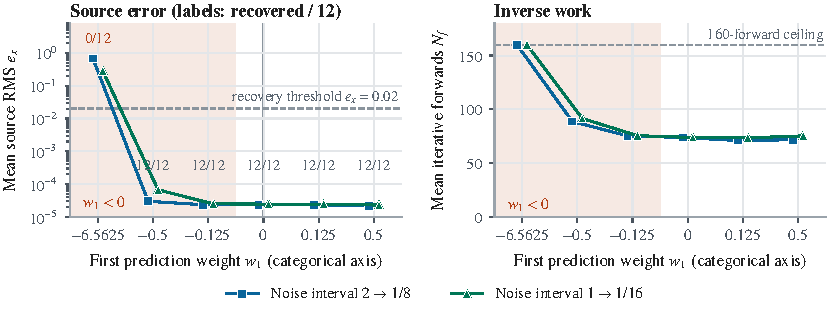
\includegraphics[width=.55\linewidth]{../figures/controlled.pdf}
\caption{The full controlled sweep on both fixed-ratio intervals (main paper Fig.~3). The weight axis is categorical; panels (a) and (c) use log scales. Numbers above (a) count recovered sources and apply to both blocks. Attained residuals and $g_{\rm err}$ are in \cref{tab:controlled}.}
\label{fig:controlled}
\end{figure}

Each of the five tested weights between $-0.5$ and $0.5$ recovers all twelve sources in both blocks. At $w_1=-0.5$ on $2\to1/8$, mean forward RMS drops from $0.0460$ to $0.0347$ relative to zero, with $14.8$ more mean iterative calls. The lower-noise block shows the same trade-off. The $-6.5625$ arm reaches the ceiling on every source and recovers none in either block. Its median $g_{\rm rand}$ is larger than at zero in both blocks.

Each arm uses its own output and target-based initializer. Across blocks, source states and absolute noise scales vary together. The Heun64/128 mean RMS differences are $1.89\times10^{-5}$ and $1.28\times10^{-5}$ for $2\to1/8$ and $1\to1/16$. The sweep used 29,120 forwards, including 13,082 iterative calls and the remaining calls for qualification, generation, references, initialization and diagnostics.
\FloatBarrier
